\tikzsetnextfilename{fig-cubic-P2mod3}
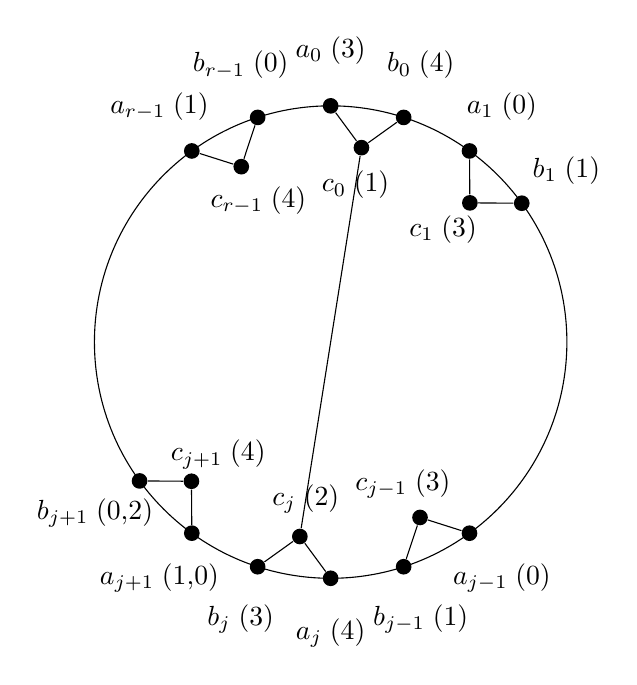
\begin{tikzpicture}[scale=1, 
    vertex/.style={circle, fill=black, inner sep=2pt}
]

% Círculo exterior
\draw (0,0) circle (3cm);

% Vértices a_i, b_i
\foreach \i/\name/\col in {
    0/$a_0$/3,  1/$b_0$/4,
    2/$a_1$/0,  3/$b_1$/1,
    %4/$a_2$/1,  5/$b_2$/2,
    %6/$a_3$/0,  7/$b_3$/1,
    8/$a_{j-1}$/0,  9/$b_{j-1}$/1,
    10/$a_j$/4, 11/$b_j$/3,
    12/$a_{j+1}$/{1,0}, 13/$b_{j+1}$/{0,2},
    %14/$a_7$/2, 15/$b_7$/3,
    %16/$a_8$/4, 17/$b_8$/2,
    18/$a_{r-1}$/1, 19/$b_{r-1}$/0}
{
    \node[vertex] (v\i) at ({90-18*\i}:3) {};
    \node [shift=({90-18*\i}:0.7)] at (v\i) {\name\;(\col)};
}

% Vértices c_i, centrados entre a_i y b_i
\foreach \i/\name/\col in {
    0/$c_0$/1, 1/$c_1$/3,
    %2/$c_2$/3, 3/$c_3$/4,
    4/$c_{j-1}$/3, 5/$c_j$/2,
    6/$c_{j+1}$/4,
    %7/$c_7$/0, 8/$c_8$/0,
    9/$c_{r-1}$/4}
{
    % \node[vertex] (c\i) at ({81-36*\i}:2.2) {};
    \node[vertex] (c\i) at ({81-36*\i}:2.5) {};
    \node [shift=({81-36*\i}:-0.48)] at (c\i) {\name\;(\col)};
}

% Aristas a_i-c_i y b_i-c_i
\foreach \i in {0,1,4,5,6,9}
% \foreach \i in {0,1,2,6,7,8}
{
    \pgfmathtruncatemacro{\a}{2*\i}
    \pgfmathtruncatemacro{\b}{2*\i+1}
    \draw (v\a)--(c\i)--(v\b);
}

% Aristas del matching M
\draw (c0)--(c5);
%\draw (c2)--(c3);
%\draw (c4)--(c5);
%\draw (c6)--(c7);
%\draw (c8)--(c9);

\end{tikzpicture}